\chapter{Framework implementation}
\label{chap:implementation}

The API, as described in chapter \ref{chapter:api}, and the decision making logic from chapter \ref{chap:deciding} was implemented into the ScalaAdaptive framework, a simple library that can be added to any Scala project and allows the programmer to utilize the adaptive decision making in his application.

In this chapter, we will go through the implementation of the framework, its basic architecture and extensibility

\section{Goals of implementation}

The main concerns upon implementing the library were the following:

\begin{itemize}
	\item To separate the API from the selection logic
	\item To keep the library strongly typed and use static type checking even in the internal parts of the code
	\item To make the library as extensible as possible
	\item To keep the library overhead as low as possible
	\item To keep the code well-organized, to minimize code duplication
\end{itemize}

\subsubsection{Development approach}

The main development approach was to use the Scala language features to make the code simpler, easier to maintain and less error-prone. We tried to benefit from the functional approach whenever possible, while still keeping the high-level design object oriented. It leads to having the data and functionality separated in different classes. Inheritance is used only for implementing traits (except for some special cases, like the API function objects) and composition is preferred in general. All of the functionality-providing classes are used via corresponding traits, and thus communicating only through a simple and limited interface, which allows replacing them very easily.

\subsubsection{Error handling}

The library is designed so that the number of exceptions handled in the code was minimized. The library itself doesn't raise any exceptions in case of errors, and catches most of the exceptions from the libraries within to replace them with a None return value.

This approach is known from the functional programming and takes advantage of monadic operations over the \textit{Option monad}\footnote{In Haskell and other languages known as Maybe monad.}. The return values can be mapped over using the \textit{bind} operator, which allows smooth function chaining and the error propagation through the chain.

\section{Architecture overview}

This section will provide brief overview of the entire framework architecture and related decisions. More detailed description at the level of individual classes can be found in the documentation.
%TODO: Documentation reference

\subsection{API architecture}

As briefly described in section \ref{subsec:api_implementation}, the public API of the framework is represented by a set of traits \inlinecode{MultiFunction0}, ..., \inlinecode{MultiFunction5}, which expose all the user accessible methods. Because only some of the methods depend on the number of input arguments, the part of the API that can be generalized was extracted into a common trait \inlinecode{MultiFunctionCommon}, which is parametrized by the function type that extends it. 

The \inlinecode{MultiFunctionN} traits are implemented by a set of classes called \inlinecode{FunctionAdaptorN}. This is the default implementation directly inaccessible to the user. This separation allows us to modify or extend the internal API of the \inlinecode{FunctionAdaptorN} classes without changing the public API. The methods that can be implemented independently on the number of input arguments are implemented in an abstract class \inlinecode{FunctionAdaptorBase} that the other classes inherit from.

It would be quite impractical to manipulate with N different classes that represent the combined functions inside the internal parts of the framework. Therefore, the actual class holding the functions, \inlinecode{CombinedFunction}, is wrapped inside each one of the \inlinecode{FunctionAdaptorN} and is parametrized by the tuple type consisting of all the N arguments of the original function, and by the return type. All the functions are converted into functions of type \inlinecode{(TArgType) => TRetType} in the following way:

\lstset{style=Scala}
\begin{lstlisting}
val tupleFunction = (tupleArg) => function(tupleArg._1, ..., tupleArg._n)
\end{lstlisting}
	
The whole inner part of our framework works only with these \inlinecode{CombinedFunction} types and therefore with functions of type \inlinecode{(TArgType) => TRetType}. Individual function adaptor classes perform the composition of the arguments into the tuple version before propagating the call further whenever a method depending on the argument number is invoked.

The figure \ref{fig:inheritance_function_adaptors} shows this inheritance scheme.

\begin{figure}[h!]
	\captionsetup{justification=centering,margin=0.5cm}
	\centerline{\mbox{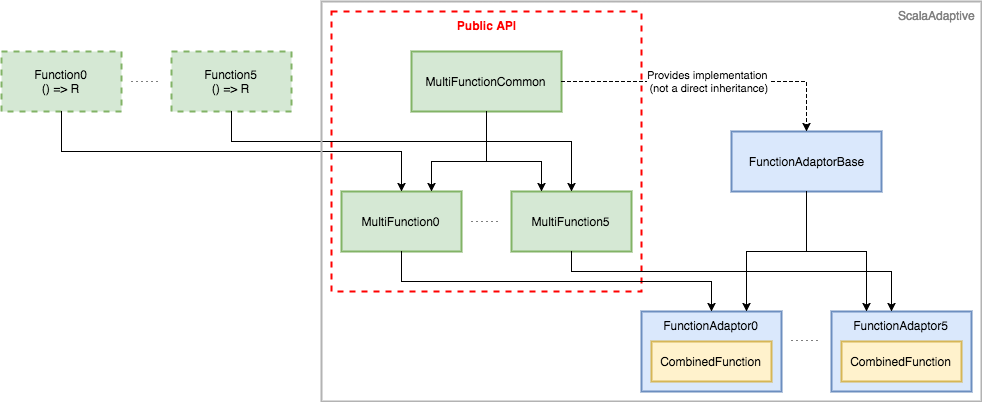
\includegraphics[width=140mm]{./img/inheritance_function_adaptors.png}}}
	\caption{Diagram showing the inheritance chain of MultifFunctionN and related classes.}
	\label{fig:inheritance_function_adaptors}
\end{figure}

\subsection{Internal architecture}
\label{subsec:internal_architecture}

The simplified internal architecture can be seen in the figure \ref{fig:internal_architecture}. It shows the core chain that is executed when a combined function, represented as a \inlinecode{MultiFunctionN} to the user, but internally stored as a \inlinecode{CombinedFunction} instance, is called.

As we can see, there are two principal logic units participating in the process:

\begin{enumerate}
	\item \textbf{\inlinecode{CombinedFunctionInvoker}} \\
	Supposed to make a quick decision based on the policy of the combined function. It should either directly invoke one of the functions, or delegate the call to the \inlinecode{AdaptiveSelector}, and update the statistics of the combined function afterwards. It works only with the data directly stored in the \inlinecode{CombinedFunction} instance, it does not have any state or shared storage.
	\item \textbf{\inlinecode{AdaptiveSelector}} \\
	The key component of the framework, it receives a set of functions and an input, and it should decide which one of them to run and to execute it, evaluate the function run and return the result. The default implementation works with an abstract history storage (\inlinecode{HistoryStorage}) a pair of selection strategies (\inlinecode{SelectionStrategy}) and an evaluator (\inlinecode{EvaluationProvider}).
\end{enumerate}

\begin{figure}[h!]
	\captionsetup{justification=centering,margin=0.5cm}
	\centerline{\mbox{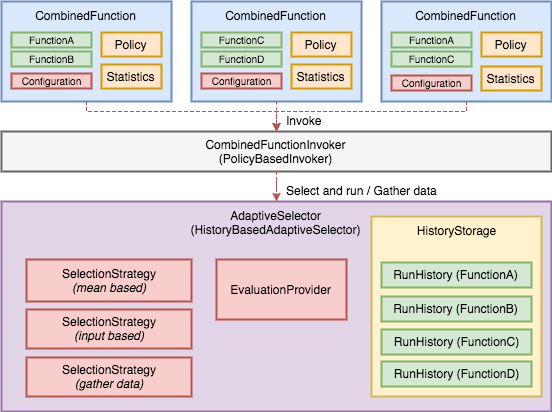
\includegraphics[width=140mm]{./img/internal_architecture.png}}}
	\caption{Diagram showing the internal architecture of the ScalaAdaptive framework.}
	\label{fig:internal_architecture}
\end{figure}

\section{Implementation options}

\subsection{HistoryStorage location}
\label{subsec:storing}

\inlinecode{HistoryStorage} is supposed to gather and store history data for all functions that are invoked using a combined function. The question is, where to save the data and how accessible to make it.

\subsubsection{Local}

First option is to make the storage part of the \inlinecode{CombinedFunction} itself. In this case, the history data would, just like the statistics, be unique for every instance of the class, i.e. for every \inlinecode{MultiFunctionN} created by the user of the library. This has two consequences:

\begin{itemize}
	\item A function will have separate histories for every use in a combined function
	\item Every new instance of a combined function will have an entirely new history for all the functions
\end{itemize}

The second consequence might lead to some unexpected behavior - for example, if we create a combined function inside of a method call as described in section \ref{subsubsec:method_from_combined_func} and call it just once, it will have a clear history every time and will be useless:

\lstset{style=Scala}
\begin{lstlisting}
def processData(data: List[Int]): Int = 
  (impl1 _ or impl2 withStorage Storage.Local)(data)
\end{lstlisting}

Some use cases for this configuration exist, e.g. if we have a class that holds some immutable data and we keep executing some computations on the data, then a combined function defined as a field on this class with local storage will adapt specifically to the data of the class and does not need input based strategies.

\subsubsection{Global}

Another option is to store all the measured data globally, in a static area of the memory accessible from all contexts. This will allow to collect run data for functions faster and share them across all the combined functions, which usually leads to more informed and more precise decisions. This is usually the preferred approach for some business logic or utility methods in long-running services. A unique identifier has to be used to match the function history record with the actual function in the \inlinecode{CombinedFunction} class. The selection of the identifier will be discussed later.

\subsubsection{Persistent}

The biggest problem of the discussed storage location is that the run history data are available only during a single run of the application. Whenever the application restarts, it will have to collect the data again. This might not be a problem for some long running services or daemons, but it is not very convenient for some tools or client applications with shorter lifecycle.

A solution to the problem is storing the data in a persistent storage, most likely on the HDD. We can do it in three different ways:

\begin{enumerate}
	\item Immediately persist each run history record
	\item Persist all of the records when the application terminates
	\item Buffer the history records and persist them in batches
\end{enumerate}

The first option seems like the best one, but it would lead to a series of I/O operations upon every invocation of a combined function. The added overhead of this solution would be dramatic. The second option, on the other hand, has no runtime overhead at all, but it requires a possibility to detect an application termination from our framework. JVM does not guarantee finalizers being called and relying on notifications from the user would complicate the API and generally be problematic. There is a mechanism in JVM called \textit{shutdown hooks} that allow the user to perform a custom action on shutdown, but it will not be called when the application crashes. Additionally, it might be unexpected from a library to perform actions on shutdown and the delay that caused by persisting a lot of run data on a slow HDD (or even a network drive) could lead to the application being terminated immediately in some automatized environments.
Therefore, the third option was selected, as it leads to the runs being regularly saved and the I/O overhead is lower.

This solution relies on the unique function identifier as well. There are additional problems connected to persisting the run history, namely:
\begin{itemize}
	\item Running multiple instances of the application at once (collisions on the persisted data file)
	\item Changes in the application code (outdated run data, changed identifiers, etc.)
	\item Having to deal with larger amounts of history data
\end{itemize}

\subsection{History storage function identifiers}
\label{subsec:function_identifiers}

As described in section \ref{subsec:storing}, we need some sort of identifier of the function to be able to store the run history data in a global or persistent storage. It does not make sense to use the references to the function objects, as new closures are created every time a lambda expression (or an eta-expanded method) is assigned.

%TODO: Reference an example?

This leaves us with three basic identifier options.

\subsubsection{Type name}

Functions in Scala are instances implementing the \inlinecode{FunctionN} trait. The default implementations are anonymous closure classes that are compiled from lambda expressions. Two different functions originated in two different lambda expressions and thus have two different type names, the ones that were generated and assigned by the compiler. The fully qualified type name can be used as the identifier of a function

Using the type names as unique identifiers is safe and straightforward. A small disadvantage is that they aren't very readable, the compiler uses the name of the type that contained the lambda expression followed by sequential number. 

There is also a subtle danger connected - if we try to combine two different function that originated from the same lambda expression (the difference might be determined by the closure arguments), they will have the same identifier, thus sharing the same history, which is usually not desirable.

The next problem is that in case of persisting the run history, the closure classes might get renamed automatically upon recompiling. The compiler usually assigns the closure names sequentially, so this could happen by just inserting another lambda expression into the enclosing class code before the current one. Run history data might even get mixed up as the newly added lambda expression could have the former name of the original closure (by taking its position in the sequence).

If the \inlinecode{FunctionN} trait has a different than default implementation, the type name identification might fail - the trait can be implemented by a single class wrapping other values. In this case, all functions implemented by that class would share the run history.

Last but not least, every time a method gets eta-expanded, a new lambda expression with new type name is generated, so in the following case, the \inlinecode{method1} would not have the same identifier in the two combined functions:

\lstset{style=Scala}
\begin{lstlisting}
val fun1 = method1 _ or method2
val fun2 = method1 _ or method3
\end{lstlisting}

\subsubsection{Method name}
\label{subsec:methodnameident}

The most common usage pattern is the one where the functions used with the \inlinecode{or} method are \textit{eta-expanded} methods (see \ref{subsubsec:apimethods}). It would be handy to use the method name as an identifier in such a case, which would lead to a better readability and allow the same method used in different combined functions to have just one run history.

The problem is that at runtime, the implicit type conversion method or the \inlinecode{or} method will always get the already \textit{eta-expanded} function object with a compiled \inlinecode{apply} method. The names have to be extracted at compile time, using the def macros (see \ref{sec:defmacros}). At the moment of implicit conversion from \inlinecode{FunctionN} to \inlinecode{FunctionAdaptorN}, the AST\footnote{Abstract syntax tree.} of the \inlinecode{FunctionN} expression can be examined - if it's a lambda expression containing one method call, the method name can be extracted.

\subsubsection{Custom identifier}
\label{subsubsec:custom_identifier}

In order to handle the specific cases where type name and method name identifiers do not distinguish correctly between different functions, there is also a possibility of choosing a custom, arbitrary identifier. This has to be triggered specifically by the user in the API and should be used in the cases where:

\begin{enumerate}
	\item User knows that the automatically assigned identifiers will not be sufficient
	\item User wants to replace default type identifier with custom identifier because of readability
\end{enumerate}

\section{Extracting method name from eta-expansion AST}

We would like to extract the method name in the process of conversion from \inlinecode{FunctionN} to the \inlinecode{MultiFunctionN}. To achieve that, we are going to have to modify the conversion process in the following way:

\begin{enumerate}
	\item Replace the implicit conversion method from \inlinecode{FunctionN} to \inlinecode{FunctionAdaptorN} by a def macro (see \ref{sec:defmacros}) and extract the conversion logic into a different, non-implicit method (in our case, the Conversions singleton object methods \inlinecode{toAdaptor()})
	\item Inside the macro, analyze the AST, detect eta-expansion method call
	\item If there is a method call:
	\begin{enumerate}
		\item Generate the identifier expression as a \inlinecode{getTypeName} call on the target of the method call, followed by the method name
		\item Generate the conversion code with explicitly specified reference expression
	\end{enumerate}
	\item Otherwise generate the conversion code with implicit reference	
\end{enumerate}

The conversion is done using the \inlinecode{toAdaptor()} method with two overloads:
\begin{itemize}
	\item Accepting only the function - implicit reference is used (type name of the closure)
	\item Accepting the function and a custom reference - the reference provided is used
\end{itemize}

\subsection{Eta-expansion AST format}

First step in the macro implementation has to be parsing the input AST and detecting patterns that are generated from eta-expansions by the compiler. Using the \inlinecode{printAst()} macro mentioned in \ref{subsec:buildingast}, the following facts were discovered:

\begin{itemize}
	\item The eta-expansion is already replaced by the equivalent code in AST, so it can't be detected directly.
	\item The result of eta-expansion is a lambda expression (function literal).
\lstset{style=Dump}
\begin{lstlisting}
Function(...)
\end{lstlisting}
	\item The lambda expression is always wrapped in a block, being its return value.
	
\lstset{style=Dump}
\begin{lstlisting}
Block(
  List(...), 
  Function(...))
\end{lstlisting}	
	
	\item If the target of the invocation is either a constant or \textit{this}, it is captured in the lambda expression closure (i.e., the constant or \textit{this} is referenced directly from the function body).
	
	\item If the target of the invocation is a variable or a result of a more complicated expression, it is extracted to the enclosing block, its result is stored in a variable local to the block and then captured in the lambda expression closure. The reason is probably to avoid multiple evaluation of expressions with possible side-efects upon every invocation of the resulting function, and to avoid the target being changed throughout the lifetime of the function. The following example shows the target being a result of an expression \inlinecode{this.getInstance()} on a \inlinecode{Class} class.
	
\lstset{style=Dump}
\begin{lstlisting}
Block(
  List(
    ValDef(
      Modifiers(SYNTHETIC), 
      TermName("eta$0$1"), 
      TypeTree(), 
      Apply(
        Select(
          This(
            TypeName("Class")), 
          TermName("getInstance")), 
        List()))), 
  Function(...))
\end{lstlisting}

	\item The function node contains argument definition and the expression itself, which is a single function application.

\lstset{style=Dump}
\begin{lstlisting}
Function(
  List(
    ValDef(
      Modifiers(PARAM | SYNTHETIC), 
      TermName("arg"), 
      TypeTree(), 
      EmptyTree)), 
  Apply(...))
\end{lstlisting}
\end{itemize}

This has a few consequences for our case. We need to generate our conversion and method retrieval code into the block return value, because we need to be able to access the invocation targets that can be defined in the block itself. The target and the method name will always be in the single Apply node representing the function body.

If the method doesn't accept any type arguments, the tree is quite simple:

\lstset{style=Dump}
\begin{lstlisting}
Apply(
  Select(
    ...invocation target expression..., 
    TermName("methodName")), 
  List(...function arguments...))
\end{lstlisting}

Where the \textit{invocation target expression} can have multiple forms based on the original expression, and can depend on the enclosing block variables. It isn't, however, important for us, as we can work with the expression as whole. The function arguments are not needed either.

If the method is generic, the type arguments need to be applied in order to convert it to a function (which can't be generic). In this case, the tree gets a little more complicated:

\lstset{style=Dump}
\begin{lstlisting}
Apply(
  TypeApply(
    Select(
      ...invocation target expression..., 
      TermName("genericMethod")), 
    List(...type arguments...))), 
  List(...function arguments...))
\end{lstlisting}

The method call is wrapped in a TypeApply node before being invoked using the Apply node. The TypeApply node can in our case be ignored.

And the most complicated case we can encounter is when the method has some implicit arguments as well:

\lstset{style=Dump}
\begin{lstlisting}
Apply(
  Apply(
    TypeApply(
      Select(
        ...invocation target expression...,
        TermName("genericMethodImplicit")), 
      List(...type arguments...)), 
    List(...function arguments...)), 
  List(...implicit arguments...))
\end{lstlisting}

One more Apply node is added to the topmost level - the implicit arguments are applied after applying the actual function arguments. Their definition contains another nested block and lambda expression, but again, it is not necessary for our case. We just need to extract the invocation target and the method name.

\subsection{Generating the conversion}
\label{subsec:generate_conversion}

Supposing we have the invocation target expression and the method name, we need to create the identifier string expression that will be used in the manual \inlinecode{toAdapter} invocation.

In order to extract the fully qualified name of the method call target, we need to generate the following expression:

\lstset{style=Scala}
\begin{lstlisting}
invocationTarget.getClass.getTypeName + ".methodName"
\end{lstlisting}

The AST representing this expression has to be wrapped in the \inlinecode{MethodNameReference} construction application (it is a case class with automatically generated \inlinecode{apply()} method) to get the resulting reference.

In all the cases, the \inlinecode{toAdapter} method has to be generated to replace the macro function. The function literal from the original AST has to be passed in as the first argument, and optionally, the second argument can be provided if the extraction of the method name was successful.

The original tree in a simplified form can be seen in figure \ref{fig:original_eta_ast}.

\begin{figure}[h!]
	\captionsetup{justification=centering,margin=0.5cm}
	\centerline{
		\begin{forest}
			[Block
			[Statements
			[ValDef]
			]
			[Function]
			]
		\end{forest}
	}
	\caption{The original simplified eta-expansion AST.}
	\label{fig:original_eta_ast}
\end{figure}

We need to transform the block, keeping the definition in the statement part, but wrapping the \inlinecode{Function} into the \inlinecode{toAdapter} call, as shown in figure \ref{fig:transformed_eta_ast}.
	
\begin{figure}[h!]
	\captionsetup{justification=centering,margin=0.5cm}
	\centerline{
		\begin{forest}
			[Block
			[Statements
			[ValDef]
			]
			[Apply
			[toAdaptor]
			[ArgumentList
			[Function]
			[ExtractedReferenceExpression]
			]
			]
			]
		\end{forest}
	}
	\caption{The simplfied eta-expansion AST after manually adding toAdaptor call.}
	\label{fig:transformed_eta_ast}
\end{figure}

\subsection{Extracting method overloads}

The approach that was described so far has one small issue - it doesn't recognize function overloads, so all the overloads share the same identifier.

 It wouldn't be difficult to extract the actual number of arguments that the method is being invoked with and include it in the reference. When attempting to extract the argument types of the lambda expression, we encounter a major problem - the function literal is generated without argument type specification, the TypeTree is empty:

\lstset{style=Dump}
\begin{lstlisting}
ValDef(
  Modifiers(PARAM | SYNTHETIC), 
  TermName("i"), 
  TypeTree(), 
  EmptyTree)
\end{lstlisting}

This can be done and is quite similar to the following piece of code:

\lstset{style=Scala}
\begin{lstlisting}
val function: (Int) => Int = { i => math.abs(i) + 1 }
\end{lstlisting}

In this case, the lambda expression doesn't have the type of its arguments specified either, because the compiler will infer it from the context in which the expression is used, in this case, from the type specifier of the variable.

The compiler is able to infer the data type from the usage of the argument as well:
\lstset{style=Scala}
\begin{lstlisting}
def method(i: Int): Int = ???
val function = { i => method(i) }
\end{lstlisting}

The previous piece of code is correctly compiled by the Scala compiler, although some IDEs (namely IntelliJ IDEA 2016.3.4) aren't able to infer the type and mark the code as incorrect.

Note that the eta-expansion is guided by the same rules, so whenever expanding a method without overloads, the compiler infers the types by itself:
\lstset{style=Scala}
\begin{lstlisting}
def method(i: Int): Int = ???
val function = method _
\end{lstlisting}

Upon expansion of a method with overloads, the resulting function type has to be provided and the inference flow goes in the other direction:
\lstset{style=Scala}
\begin{lstlisting}
def method(i: Int): Int = ???
def method(s: String): Int = ???
val function: (String) => Int = method _
\end{lstlisting}

As a consequence, at the time of syntax analysis, the types aren't inferred yet and there is no way for us to find out which method overload is being called.

The method overloads have to share the same identifier, but in most typical cases, this isn't a problem. Otherwise, it can be solved by using custom identifiers.

\subsection{The conversion demonstration}

As a practical demonstration of the process described in this section, we are going to show the compile-time conversions that are done on a method identifier that is being \textit{eta-expanded} and converted into a \inlinecode{MultiFunctionN}. Let's consider the following code:

\lstset{style=Scala}
\begin{lstlisting}
val combined1 = target.method _ or function2
\end{lstlisting}

We will follow the conversions that the compiler and our macro perform on the \inlinecode{target.method \_} expression\footnote{The actual changes are performed on the AST level, we will show them in corresponding Scala code for simplicity.}:

\begin{enumerate}
	\item The explicit \textit{eta-expansion} is done:
	\lstset{style=Scala}
	\begin{lstlisting}
{ () => target.method() }
	\end{lstlisting}
	\item The implicit conversion is applied:
		\lstset{style=Scala}
	\begin{lstlisting}
Implicits.toMultiFunction0({ () => target.method() })
		\end{lstlisting}
		\item The macro \inlinecode{toMultiFunction0} is executed and expanded:
		\lstset{style=Scala}
		\begin{lstlisting}
Conversions.toAdaptor({ () => target.method() }, MethodNameReference(this.getClass.getName + ".method"))
		\end{lstlisting}
\end{enumerate}

The final state shows the code that will be present in our compiled program and will be executed.

\subsection{Macros in the combining method}

In the section \ref{subsubsec:apimethods}, we explained why the \inlinecode{or} method has to accept an argument of \inlinecode{FunctionN} type instead of \inlinecode{MultiFunctionN}. This does not seem to cause any trouble as we can manually convert \inlinecode{FunctionN} into the \inlinecode{FunctionAdaptorN} inside the method body. With the macro expansion, however, we run into problems. Image we do it the following way:
\lstset{style=Scala}
\begin{lstlisting}
def or(fun: (T1) => R) = orMultiFunction(Implicits.toMultiFunction1(fun))
\end{lstlisting}

The  \inlinecode{toMultiFunction1} method is a macro - it gets executed at compile time, and it receives the argument AST as its input. In this case, an AST that consists of the \inlinecode{fun} identifier. We have no way to find out, where this function will be called from and with which arguments, so in order to extract the method name, we need to convert the entire \inlinecode{or} function to a macro which will generate the conversion code just like described in section \ref{subsec:generate_conversion}, and then wrap it in the internal \inlinecode{orMultiFunction} code.

This does not require any extra AST manipulations, only one method call generations. It does, however, mean a complication - the macros cannot be called virtually. Therefore, the macro definition has to be part of the \inlinecode{MultiFunctionN} API trait, breaking somehow the encapsulation of the implementation. Fortunately, it does not perform any actions by itself, only replaces the \inlinecode{or} call with a conversion and an \inlinecode{orMultiFunction} call, which is, again, a virtual method defined on the trait without implementation and therefore encapsulated.


\section{Module implementation}
\label{sec:module_impl}

All the modules mentioned in \ref{subsec:internal_architecture} are abstract traits with replaceable implementations, that are put together using composition. The API classes have to be able to access the composed and active implementations at the moment of invocation. For this reason, a singleton Scala object \inlinecode{AdaptiveInternal} was introduced and provides a holder for the following composed modules:

\begin{itemize}
	\item AdaptiveSelector with global storage
	\item AdaptiveSelector with persistent storage
	\item CombinedFunctionInvoker
\end{itemize}

We will briefly introduce the implementations of the modules that are included in the framework.

\subsubsection{CombinedFunction}

The \inlinecode{CombinedFunction} is the main data class representing a function with multiple implementations in ScalaAdaptive. It is basically a data holder class, the important functionality was separated in order to be possible to replace. It gets created and modified when a user of the library manipulates with the \inlinecode{MultiFunctionN} API type. Part of its attributes are immutable, representing the configuration and default setup of the function, and part of its attributes are mutable, holding its state in the invocation process.

It contains the following immutable data:

\begin{itemize}
	\item Set of functions that it is combined from (wrapped into the tuple form)
	\begin{itemize}
		\item	Each function holds up to two references - one based on the closure type name, the other being either a method name or a custom name, depending on the creation process (see \ref{subsec:function_identifiers})
	\end{itemize}
	\item \textit{Descriptor function} (wrapped into the tuple form), see \ref{sec:input_based_strategies}
	\item \textit{Group selector} function (wrapped into the tuple form), see \ref{subsubsec:group_selection}
	\item A \inlinecode{FunctionConfiguration} a setup independent on the argument and return value types, consisting of the following:
	\begin{itemize}
		\item Selection strategy - Predictive or NonPredictive
		\item Storage - Local, Global or Persistent
		\item Duration - optional maximal time period for the history records
		\item ClosureReferences - if the closure type references should be preferred over the method name or the custom name
		\item Initial policy
	\end{itemize}
\end{itemize}

And the following state representing data:

\begin{itemize}
	\item Function statistics (separately for each group)
	\item Current policy (separately for each group)
	\item Analytics data - full history of all the selections and their results
\end{itemize}

In case of local storage setup, the instance also contains its own \inlinecode{AdaptiveSelector} that holds the local \inlinecode{HistoryStorage}.

\subsubsection{CombinedFunctionInvoker}

It has access to the state of the \inlinecode{CombinedFunction} and its basic implementation does the following:

\begin{itemize}
	\item Evaluate the current policy on the statistics of the combined function
	\item According to the result either invoke directly the function which is directly accessible through the statistics (the last one and the most selected one), or pass the decision onto the \inlinecode{AdaptiveSelector}
	\item Update the function statistics
\end{itemize}

The \inlinecode{AdaptiveSelector} is accessed either through the \inlinecode{CombinedFunction} itself in case of local storage setup, or using the singleton object \inlinecode{AdaptiveInternal} in case of global or persistent setup.

\subsubsection{AdaptiveSelector}

A module which is supposed to select one of given options to run, and to evaluate the run. It is parametrized with \inlinecode{TMeasurement} type, which represents the data measured from the function run. By default, a \inlinecode{Long} type for run time measured is used.

The implementation \inlinecode{HistoryBasedAdaptiveSelector} uses a \inlinecode{HistoryStorage} to store and retrieve the run data of individual functions. In addition, it holds two \inlinecode{SelectionStrategy} instances, one for the input based selection, the other for the mean based selection. One of these two instances is used to select the function to run, which is then executed using an \inlinecode{EvaluationProvider}. The measurement retrieved is added to the history and the result is returned, along with a performance benchmark including execution and overhead times (independent on the actual measurement, always based on wall-clock times) for the function statistics update. Figure \ref{fig:history_based_selector} shows the entire process.

\begin{figure}[h!]
	\captionsetup{justification=centering,margin=0.5cm}
	\centerline{\mbox{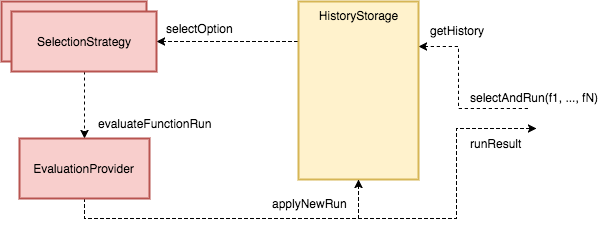
\includegraphics[width=100mm]{./img/history_based_selector.png}}}
	\caption{Diagram showing the HistoryBasedAdaptiveSelector execution path.}
	\label{fig:history_based_selector}
\end{figure}

\subsubsection{HistoryStorage}

A type with a map-like interface - it is supposed to hold \inlinecode{RunHistory} instances for each combination of function and group. A key composed of the function reference and the group identifier is used to access the histories.

There are two implementations in the framework:

\begin{itemize}
	\item \inlinecode{MapHistoryStorage} - stores the histories in memory
	\item \inlinecode{PersistentHistoryStorage} - a wrapping storage that delegates the calls to an internal \inlinecode{HistoryStorage}, and, in addition, it serializes every new run to a \inlinecode{HistorySerializer} and if asked for a history that is not present in the underlying storage, it tries to deserialize it using the same class
\end{itemize}

The \inlinecode{HistorySerializer} has two basic implementations, one for direct serialization, and one for buffered serialization. The data are stored into a file, one per function, and the format, root directory and file name pattern are fully customizable. There is no list of these history containing files anywhere - when trying to deserialize a function, a file with corresponding name is checked for existence. This means that the individual function histories are deserialized one by one, at the moment of the first invocation of a combined function that contains them, which might cause a delay in the first execution.

\subsubsection{RunHistory}

\inlinecode{RunHistory} represents the sequence of measurement results and other details about a function run. The interface is designed to support immutable solution - the appending methods always return an instance of the same type, which might or might not be the same object depending on the implementation. The interface provides some basic operations on the history, allows iteration over the data and appending new data (always at the end). Apart from that, it also has some methods to support precomputed or cached data for some of the selection strategies, namely statistical data and grouped averages for each input descriptor. These supporting methods can always be computed using the data available, and if the implementation of \inlinecode{RunHistory} does not support the caching or precomputation, there are \textit{mixin} traits with default implementations available.

The provided implementations of \inlinecode{RunHistory} can be chained using the \textit{Decorator} pattern to modify the behavior. The basic implementations are the following:
\begin{itemize}
	\item \inlinecode{FullRunHistory} - stores all runs in an \inlinecode{ArrayBuffer}, is mutable
	\item \inlinecode{ImmutableFullRunHistory} - stores all runs in an immutable \inlinecode{List}, is a little slower in general
\end{itemize}

These instances can be wrapped in the following decorator classes:
\begin{itemize}
	\item \inlinecode{LimitedRunHistory} - limits the maximum number of stored items, whenever it reaches maximum, it throws the older half of all the records away
	\item \inlinecode{CachedStatisticsRunHistory} - stores the statistical data about the run items, speeds up some selection strategies
	\item \inlinecode{CachedGroupedRunHistory} - stores average evaluation data for each \textit{run selector}, speeds up some selection strategies
\end{itemize}

\subsubsection{SelectionStrategy}

Very simple trait that represents the selection strategies described in detail in sections \ref{sec:input_based_strategies} and \ref{sec:mean_based_strategies}. The implementations should be stateless and should work only with the \inlinecode{RunHistory} records that it receives (in order not to mix together decisions about two separate history storage locations). The strategy implementations often have a customizable fallback strategy that is used in cases where the current strategy is not able to make a decision.

The strategies are parametrized by the \inlinecode{TMeasurement} type of the function run evaluation. All of the implemented strategies work with function run time represented by \inlinecode{Long}.

Implemented strategies are:
\begin{itemize}
	\item \inlinecode{LowRunAwareSelectionStrategy} - if any of the functions has less than a specified number of history records, uses one strategy, otherwise, uses a different strategy
	\item \inlinecode{LeastDataSelectionStrategy} - uses the function with least historical runs
	\item \inlinecode{TTestSelectionStrategy} - implements the t-test strategy described in section \ref{subsec:t_test_multiple}, uses the \inlinecode{org.apache.commons.math3} library
	\item \inlinecode{LimitedRegressionSelectionStrategy} - implements the window-bound linear regression strategy (the window being optional) as described in section \ref{subsec:window_bound_regression}, uses the \inlinecode{org.apache.commons.math3} library
	\item \inlinecode{LoessInterpolationSelectionStrategy} - implements the local regression strategy from section \ref{subsec:local_regression}, uses the \inlinecode{org.apache.commons.math3} library
\end{itemize}

The common composition pattern is to use the \inlinecode{LowRunAwareSelectionStrategy} as the topmost one, the \inlinecode{LeastDataSelectionStrategy} as the fallback strategy, and to have one of the actual input based or mean based strategies in the middle.

\subsubsection{EvaluationProvider}

With a goal of potentially supporting larger variety of possible function evaluation criteria, the selected function is always executed using an implementation of \inlinecode{EvaluationProvider}, which is supposed to run the function and to evaluate it, and return both the result of the function and the evaluation data in the form of \inlinecode{TMeasurement}. The default implementation simply measures the wall-clock time of the function run.

\section{Configuration and customization}

The basic behavior of the combined functions can be changed in two ways:
\begin{itemize}
	\item Each combined function can have the most basic features configured
	\item The whole framework can be re-configured and customized
\end{itemize}

\subsection{Composed function configuration}

There is a fluent and simple way to configure the most basic behavior as part of the function composition API (see section \ref{subsec:api_function_configuration}). It is based mostly on selecting which one of multiple implementation options should be used with given function. In the \inlinecode{AdaptiveInternal} singleton, we hold two implementations of \inlinecode{AdaptiveSelector}, one with persistent history storage, the other without. Each of these two implementations then includes two instances of  \inlinecode{SelectionStrategy}, one for input based and one for mean based selection.

The function configuration methods and possible values are the following:

\begin{itemize}
	\item \inlinecode{storeUsing} - represents the history storage options as described in section \ref{subsec:storing}
	\begin{itemize}
		\item \inlinecode{Global} - uses the shared \inlinecode{AdaptiveSelector} without persistent storage
		\item \inlinecode{Persistent} - uses the shared \inlinecode{AdaptiveSelector} with persistent storage
		\item \inlinecode{Local} - creates a new instance of \inlinecode{AdaptiveSelector} locally in the function object
	\end{itemize}
\item \inlinecode{selectUsing}
\begin{itemize}
	\item \inlinecode{InputBased} - uses the input based strategy from the \inlinecode{AdaptiveSelector}
	\item \inlinecode{MeanBased} - uses the mean based strategy from the \inlinecode{AdaptiveSelector}
\end{itemize}
\item \inlinecode{limitedTo} - allows to specify the maximum age of the history records to be used in the selection process
\item \inlinecode{asClosures} - represents the history storage identifier choice as described in section \ref{subsec:function_identifiers}
\begin{itemize}
	\item \textit{true} - always uses closure type names as the function references
	\item \textit{false} - uses either method names or custom names as the function references if available
\end{itemize}
\item \inlinecode{withPolicy} - allows to specify the starting policy for the function
\end{itemize}

The user of the library is expected to specify this configuration with most of the combined functions. Especially the choice between the input based and mean based strategy is very important.

\subsection{Framework configuration}
\label{subsec:framework_config}

In section \ref{sec:module_impl}, we mentioned a variety of building blocks that the main parts of the framework are composed of, and the possibility to use multiple implementation to change the behavior of the entire system. This is the more advanced part of the configuration and it requires manipulation with the actual implementations.

As explained earlier, all the shared and commonly accessible functionality is held inside the singleton object \inlinecode{AdaptiveInternal}. This object can be initialized using an \inlinecode{initialize()} method on a publicly accessible singleton \inlinecode{Adaptive}. The static description of the composition of the implementations that is followed in this process is provided by a \inlinecode{Configuration} trait. This can be though of as a composition root of the whole system - it has to provide factory functions for all the building blocks used. In addition, it has an abstract type member \inlinecode{TMeasurement} for the evaluation data. 

%TODO: Add ref to http://docs.scala-lang.org/tutorials/tour/abstract-types.html

The implementation of the \inlinecode{Configuration} trait has to specify the \inlinecode{TMeasurement} type and provide the factory methods which are already specific for the type. Note that the \inlinecode{AdaptiveSelector} trait and its methods do not depend on the \inlinecode{TMeasurement}, only its implementation does, so the type of the evaluation data does not leak outside of the composition root. As a result, the actual type can be changed at runtime by simply replacing the \inlinecode{AdaptiveSelector} implementation.

The \inlinecode{Configuration} can be created by the user himself, using either a combination of provided implementation or his own implementations. Alternatively, one of the predefined \inlinecode{Configuration} types can be utilized:

\begin{itemize}
	\item \inlinecode{BaseConfiguration} - provides basic configuration of the types that do not depend on the \inlinecode{TMeasurement}
	\item \inlinecode{BaseLongConfiguration} - sets the \inlinecode{TMeasurement} type to \inlinecode{Long} and add basic configuration of the types that depend on it
\end{itemize}

These traits can be extended and customized by overriding some of the functions.

\subsubsection{Configuration blocks}
 To simplify the configuration process when working with existing implementations and to hide the initialization details from the user, a concept called \textit{configuration blocks} was introduced. 
 
 \textit{Configuration blocks} are traits that provide implementation for just one (or a few) functions from the \inlinecode{Configuration} trait, setting up part of the framework in given way. The user of the framework can then define the configuration by creating an anonymous class extending the base configuration along with desired \textit{configuration blocks}. Thanks to the fluent and simple syntax of Scala, this concept is very expressive and easy to use. The compile-time check will automatically alert the user if the combination of block does not cover some required method.
 
 In addition, some blocks can be parametrized. The parameters are always protected read-only attributes of the block trait that usually have default implementation (i.e. value), but can be overridden. It fits easily into the anonymous class usage pattern, as the new parameter values for all the blocks can simply be stated in the body of the class. Blocks can share a parameter by inheriting it from the same base trait - in such a case, it is impossible to set different values for different blocks.
 
 The whole configuration can look the following way:

\lstset{style=Scala}
\begin{lstlisting}
val config = new BaseLongConfiguration
  with DefaultHistoryPath
  with RunTimeMeasurement
  with WindowBoundRegressionInputBasedStrategy
  with UTestMeanBasedStrategy
  with CachedRegressionAndStatisticsStorage
  with FileLogging {
  override val maximumNumberOfRecords = 20000
  override val alpha = 0.25
  override val logFilePath = "./adaptive/log.txt"
}

Adaptive.initialize(config)
\end{lstlisting}

List of all the configuration blocks available along with their parameters can be found in appendix REF.

%TODO: Update blocks AND add block params!

\subsubsection{Default configuration}

A special class for the default configuration was created, which is used to initialize the ScalaAdaptive framework at the beginning of the application run and which provides the implementations that are used if the user does not provide his configuration.

Based on the results observer in section \ref{sec:strategy_comparison}, we decided to include the t-test selection strategy with cached statistics as the mean based strategy, and the window-bound linear regression as the input based strategy.

The default configuration can be extended with any of the configuration blocks as well:

\lstset{style=Scala}
\begin{lstlisting}
val config = new DefaultConfiguration with ConsoleLogging
\end{lstlisting}

\subsection{Extending the framework}

The framework can be simply extended without actually modifying it by creating custom implementations of some of the traits that are used by the invocation and selection process, and by supplying it to the \inlinecode{Adaptive} initialization using a custom configuration, as described in \ref{subsec:framework_config}.

An overview of the areas that are the simplest and most useful to extend will follow.

\subsubsection{Selection strategies}

A new selection strategy can be created by implementing the \inlinecode{SelectionStrategy} trait and by providing the implementation as either input based or mean based selection strategy. The trait itself is technically a single function which is given a sequence of function run histories and an input descriptor and is supposed to return the run history of the function with best expected performance:

\lstset{style=Scala}
\begin{lstlisting}
def selectOption(records: Seq[RunHistory[TMeasurement]], 
  inputDescriptor: Option[Long]): RunHistory[TMeasurement]
\end{lstlisting}

The strategy will most likely have to work with either a specific evaluation data type, or at least put a constraint on it (by using the \textit{viewability} mechanism, see section \ref{subsec:implicit_args}).

\subsubsection{History storages}

If we wanted to change the way in which the history data are stored, e.g. by filtering some of the results, performing some aggregations to save space, etc., we would need to implement one or both of the following traits - the \inlinecode{RunHistory} trait, that represents the sequence of results for one group and function, and the \inlinecode{HistoryStorage} trait, that manages the \inlinecode{RunHistory} instances for different groups and functions.

The main advantage is that these implementations can work with unspecified evaluation data type, if they are supposed to work just like a storage, or to have a fixed evaluation data type in case when some data aggregations or precomputations are required.

\subsubsection{Evaluation data}

We can change the \inlinecode{TMeasurement} data type and make the framework perform the adaptations according to a different (or more complex) evaluation results. In such a case, we need to implement the \inlinecode{EvaluationProvider} trait, and then add our custom selection strategies that select based on the new evaluation type.